\documentclass{article}

\usepackage[margin=1in]{geometry}
\usepackage{amsmath}
\usepackage{mathtools}
\usepackage{graphicx}
\usepackage{float}

\title{Multiplication Problems}
\author{Name: \_\_\_\_\_\_\_\_\_\_\_}
\date{2022-07-17}

\begin{document}
\maketitle

\begin{figure}[H]
    \centering
    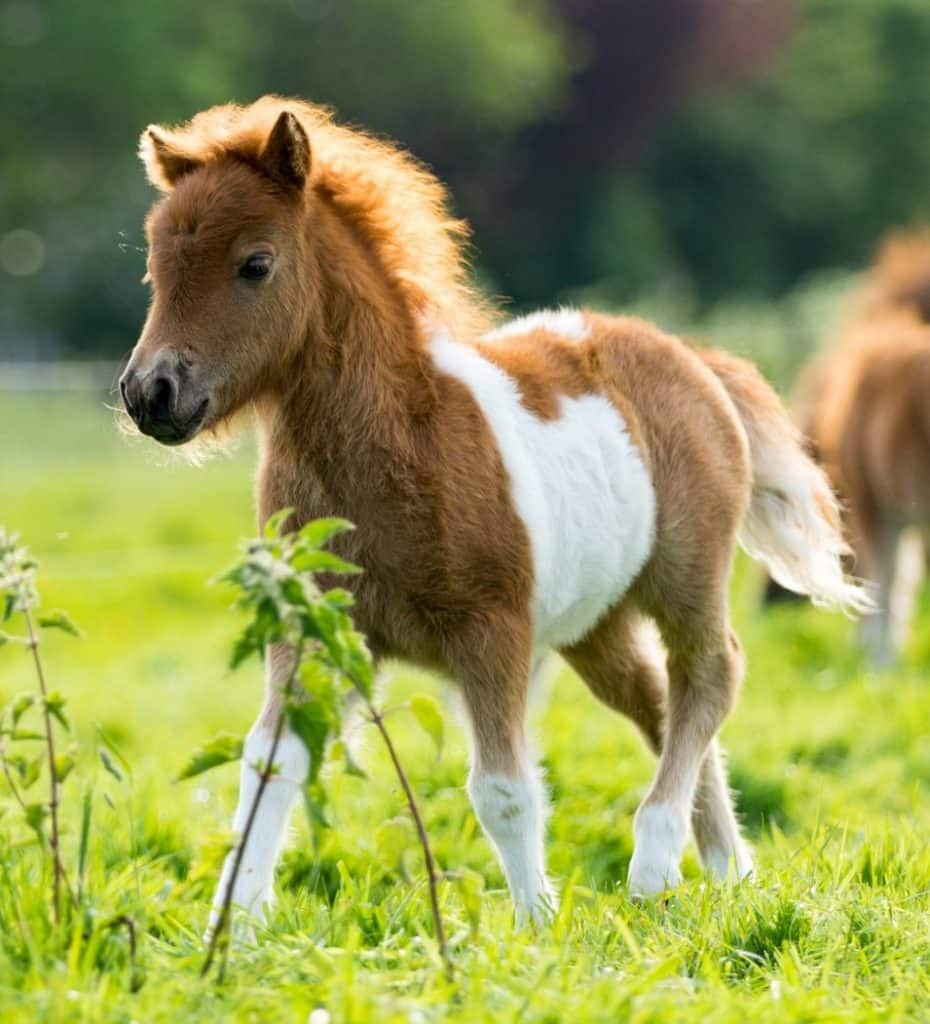
\includegraphics[width=0.2\linewidth]{images/horse.jpg}
\end{figure}

\section{Set 1}
Warmup problems

\begin{flalign*}
    20 \times 9 &= &\\
    14 \times 5 &= &\\
    10 \times 9 &= &\\
    17 \times 0 &= &\\
    13 \times 5 &= &\\
    15 \times 9 &= &\\
    11 \times 0 &= &\\
    14 \times 3 &= &\\
    14 \times 0 &= &\\
    10 \times 3 &= &
\end{flalign*}

\newpage

\section{Set 2}
One digit multiplied by three digit

\begin{tabular}{ccccc}
    \begin{minipage}{0.2\linewidth}
        \begin{table}[H]
            \begin{tabular}{c@{\,}c@{\,}c@{\,}c}
                & 1 & 3 & 5 \\
                × &   &   & 4 \\
                \hline
                \\
                \hline
                \\
                \hline
                \\
                \hline
            \end{tabular} \\
        \end{table}
    \end{minipage} &

    \begin{minipage}{0.2\linewidth}
        \begin{table}[H]
            \begin{tabular}{c@{\,}c@{\,}c@{\,}c}
                & 1 & 8 & 8 \\
                × &   &   & 4 \\
                \hline
                \\
                \hline
                \\
                \hline
                \\
                \hline
            \end{tabular} \\
        \end{table}
    \end{minipage} &

    \begin{minipage}{0.2\linewidth}
        \begin{table}[H]
            \begin{tabular}{c@{\,}c@{\,}c@{\,}c}
                & 8 & 0 & 7 \\
                × &   &   & 6 \\
                \hline
                \\
                \hline
                \\
                \hline
                \\
                \hline
            \end{tabular} \\
        \end{table}
    \end{minipage} &

    \begin{minipage}{0.2\linewidth}
        \begin{table}[H]
            \begin{tabular}{c@{\,}c@{\,}c@{\,}c}
                & 6 & 9 & 5 \\
                × &   &   & 7 \\
                \hline
                \\
                \hline
                \\
                \hline
                \\
                \hline
            \end{tabular} \\
        \end{table}
    \end{minipage} &

    \begin{minipage}{0.2\linewidth}
        \begin{table}[H]
            \begin{tabular}{c@{\,}c@{\,}c@{\,}c}
                & 2 & 2 & 9 \\
                × &   &   & 4 \\
                \hline
                \\
                \hline
                \\
                \hline
                \\
                \hline
            \end{tabular} \\
        \end{table}
    \end{minipage} \\

    \begin{minipage}{0.2\linewidth}
        \begin{table}[H]
            \begin{tabular}{c@{\,}c@{\,}c@{\,}c}
                & 5 & 4 & 5 \\
                × &   &   & 9 \\
                \hline
                \\
                \hline
                \\
                \hline
                \\
                \hline
            \end{tabular} \\
        \end{table}
    \end{minipage} &

    \begin{minipage}{0.2\linewidth}
        \begin{table}[H]
            \begin{tabular}{c@{\,}c@{\,}c@{\,}c}
                & 8 & 7 & 6 \\
                × &   &   & 8 \\
                \hline
                \\
                \hline
                \\
                \hline
                \\
                \hline
            \end{tabular} \\
        \end{table}
    \end{minipage} &

    \begin{minipage}{0.2\linewidth}
        \begin{table}[H]
            \begin{tabular}{c@{\,}c@{\,}c@{\,}c}
                & 2 & 0 & 9 \\
                × &   &   & 3 \\
                \hline
                \\
                \hline
                \\
                \hline
                \\
                \hline
            \end{tabular} \\
        \end{table}
    \end{minipage} &

    \begin{minipage}{0.2\linewidth}
        \begin{table}[H]
            \begin{tabular}{c@{\,}c@{\,}c@{\,}c}
                & 7 & 2 & 8 \\
                × &   &   & 1 \\
                \hline
                \\
                \hline
                \\
                \hline
                \\
                \hline
            \end{tabular} \\
        \end{table}
    \end{minipage} &

    \begin{minipage}{0.2\linewidth}
        \begin{table}[H]
            \begin{tabular}{c@{\,}c@{\,}c@{\,}c}
                & 6 & 3 & 1 \\
                × &   &   & 5 \\
                \hline
                \\
                \hline
                \\
                \hline
                \\
                \hline
            \end{tabular} \\
        \end{table}
    \end{minipage}
\end{tabular}

\section{Set 3}
Set 2, but with harder problems

\begin{tabular}{ccc}
    \begin{minipage}{0.33\linewidth}
        \begin{table}[H]
            \begin{tabular}{c@{\,}c@{\,}c@{\,}c@{\,}c@{\,}c}
                & 2 & 7 & 9 & 5 & 9 \\
                × & & & & & 8 \\
                \hline
            \end{tabular}
        \end{table}
    \end{minipage} &

    \begin{minipage}{0.33\linewidth}
        \begin{table}[H]
            \begin{tabular}{c@{\,}c@{\,}c@{\,}c@{\,}c}
                & 7 & 0 & 8 & 7 \\
                × & & & & 2 \\
                \hline
            \end{tabular}
        \end{table}
    \end{minipage} &

    \begin{minipage}{0.33\linewidth}
        \begin{table}[H]
            \begin{tabular}{c@{\,}c@{\,}c@{\,}c@{\,}c@{\,}c@{\,}c@{\,}c}
                & 1 & 1 & 3 & 6 & 3 & 3 \\
                × & & & & & & 7 \\
                \hline
            \end{tabular}
        \end{table}
    \end{minipage}
\end{tabular}

\end{document}